\documentclass{beamer}
\usetheme{Madrid}
\usepackage{array}
\usepackage{tikz}
\usepackage{multicol}
\usepackage{mathtools}
\title[CST 301 M4]{FORMAL LANGUAGES AND AUTOMATA THEORY}
\subtitle{Module 4}
\author{Rijin IK}
\institute[VJEC]{Assistant Professor\\Department of Computer Science and Engineering\\Vimal Jyothi Engineering College\\Chemperi}
\begin{document}
	\begin{frame}
		\titlepage
	\end{frame}
   \begin{frame}{Outline}
   \tableofcontents
   \end{frame}
\section{Course Outcomes}
\begin{frame}{Course Outcomes}
\textbf{After the completion of the course the student will be able to}
\begin{enumerate}
	\item Classify a given formal language into Regular, Context-Free, Context
	Sensitive, Recursive or Recursively Enumerable. [Cognitive knowledge
	level: Understand]
	\item Explain a formal representation of a given regular language as a finite state
	automaton, regular grammar, regular expression and Myhill-Nerode
	relation. [Cognitive knowledge level: Understand]
	\item Design a Pushdown Automaton and a Context-Free Grammar for a given
	context-free language. [Cognitive knowledge level : Apply]
	\item Design Turing machines as language acceptors or transducers. [Cognitive
	knowledge level: Apply]
	\item Explain the notion of decidability. [Cognitive knowledge level:
	Understand]
\end{enumerate}
\end{frame}
\section{Nondeterministic Pushdown Automata (PDA)}
\begin{frame}{Nondeterministic Pushdown Automata}
\textbf{Nondeterministic Pushdown Automata}
\begin{itemize}
	\item A non-deterministic pushdown automaton (NPDA), or just pushdown automaton (PDA) is a variation on the idea of a non-deterministic finite automaton (NDFA).
	\item Unlike an NDFA, a PDA is associated with a stack (hence the name pushdown).
	\item The transition function must also take into account the “state” of the stack.
\end{itemize}
\end{frame}	
\begin{frame}{Nondeterministic Pushdown Automata}
\begin{figure}
	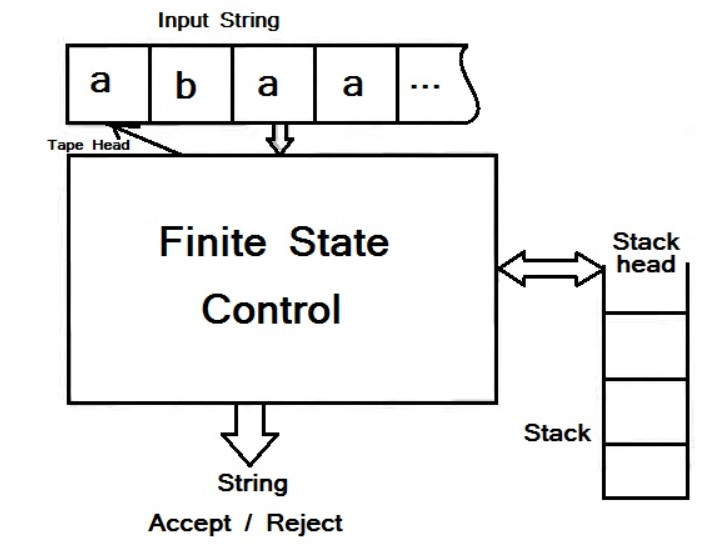
\includegraphics[scale=.7]{img4/m1}
	\caption{Block diagram of a Pushdown Automata}
\end{figure}
\end{frame}	

\begin{frame}{Nondeterministic Pushdown Automata}
	A pushdown automaton has three components
\begin{enumerate}
	\item An input tape,
		\item A control unit, and
	\item	A stack with infinite size.
\end{enumerate}
\textbf{Transition}
\begin{itemize}
	\item Read the current input symbol and the current symbol on the top of the stack
	\item Based on the \textbf{current state , current input} symbol and \textbf{current stack symbol} , change the state and replace the symbol on the top of of the stack with a string symbols
	\item After reading of a symbol from the input tape  the input tape head (read head) moves one position to the right in the input tape
\end{itemize}
\end{frame}	
\begin{frame}{Nondeterministic Pushdown Automata}
\textbf{Acceptance criteria}
\begin{enumerate}
	\item \textbf{Empty stack acceptance}
	\begin{itemize}
		\item Input is consumed and stack is empty
	\end{itemize}
	\item \textbf{Final state acceptance}
	\begin{itemize}
		\item Input is consumed and the PDA is in a final state
	\end{itemize}
\end{enumerate}
\end{frame}	
\begin{frame}{Nondeterministic Pushdown Automata}
	\textbf{ Formal definition of PDA }
		\begin{itemize}
			\item A Pushdown Automaton (PDA) is a seven-tuple: $M = (Q, \Sigma, \Gamma, \delta, q_0, z_0, F)$
			\begin{itemize}
				\item Q A finite set of states
				
				\item $\Sigma$ A finite input alphabet
				
					\item $\Gamma$ A finite stack alphabet
				
					\item $q_0$ The initial/starting state, $q_0$ is in Q
				
					\item $z_0$ Initial stack symbol, is in $\Gamma$
				
					\item $F\ 	$A set of final/accepting states, which is a subset of Q
				
					\item $\delta$	A transition function, where
					$$\delta: Q \times (\Sigma \cup {\epsilon}) \times \Gamma \rightarrow \  finite\  subsets\  of\  Q\  \times \Gamma^*$$
			\end{itemize}
		\end{itemize}
\end{frame}	
\begin{frame}{Nondeterministic Pushdown Automata}
	\begin{itemize}
		\item The transition function $\delta$ takes three arguments:
	\begin{enumerate}
		\item A state, in Q.
			\item An input, which is either a symbol in $\Sigma$ or $\epsilon$.
		\item A stack symbol in $\Gamma$.
	\end{enumerate}
\item $\delta(q, a, x)=(p, \gamma)$ where,
\begin{itemize}
	\item q is the state in Q
	\item a is an input symbol in $\Sigma$
	\item x is the stack symbol in $\Gamma$
	\item p is the new state
	\item $\gamma$ is a string of stack symbols
\end{itemize}
\item Stack operation
\begin{itemize}
	\item If $\gamma$ = $\epsilon$ , then the stack is popped
	\item	If $\gamma$ = x , then the stack is unchanged
	\item	If $\gamma$ = yz , then the x is replaced by z and y is pushed on to the stack
\end{itemize}
	\end{itemize}
\end{frame}	
\begin{frame}{Nondeterministic Pushdown Automata}
\textbf{Example:}Design a PDA that accepts $\{ww^R | w\  in\  (0+1)^*\}$\\
\textbf{Sln:}
\begin{itemize}
	\item $L = \{ \epsilon, 0, 1, 00, 11, 0110, 1001, .........\}$
	\item Let $M= (Q, \Sigma, \Gamma, \delta, q_0, Z_0, F)$ be the PDA
	\item Consider $M = (\{q_1, q_2\}, \{0, 1\}, \{0, 1, Z_0\}, \delta, q_1, Z_0, \phi)$
\end{itemize}
\small
\begin{eqnarray*}
	\delta(q_1,0,Z_0)&=&\{(q_1,0Z_0)\}  \\
		\delta(q_1,1,Z_0)&=&\{(q_1,1Z_0)\} \\
	\delta(q_1,0,0)&=&\{(q_1,00),(q2, \epsilon)\} \\
	\delta(q_1,1,0)&=&\{(q_1,10)\} \\
	\delta(q_1,0,1)&=&\{(q_1,01)\} \\
	\delta(q_1,1,1)&=&\{(q_1,11),(q2, \epsilon)\} \\
	\delta(q_2,0,0)&=&\{(q_2, \epsilon)\} \\
	\delta(q_2,1,1)&=&\{(q_2, \epsilon)\} \\
	\delta(q_1,\epsilon,Z_0)&=&\{(q_2, \epsilon \} \\
	\delta(q_2,\epsilon,Z_0)&=&\{(q_2, \epsilon)\} 
\end{eqnarray*}
\end{frame}	
\begin{frame}{Nondeterministic Pushdown Automata}
	\textbf{Transition diagram}
	\begin{figure}
	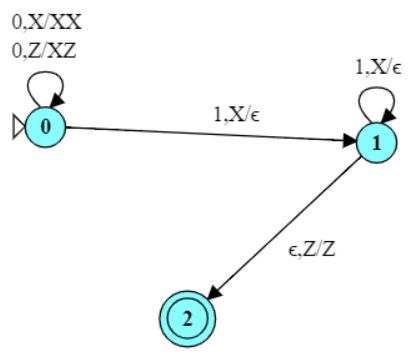
\includegraphics[scale=.7]{img4/m2}
	\caption{Transition diagram}
\end{figure}
\end{frame}	
\begin{frame}{Nondeterministic Pushdown Automata}
	\textbf{Transition diagram}
	\begin{itemize}
		\item We can show PDAs this in a transition diagram similar to the ones we used for FAs.
		\item Instead of labeling each transition with just one symbol (the input), we have to label it with three components $a,X\big|\alpha$
		where
		\begin{itemize}
			\item a	is the next input symbol.
			\item X	is the symbol the symbol at the top of the stack, where X	is one symbol of $\Gamma$
			\item	$\alpha$ is a string of stack symbols that are to be pushed onto the stack (after popping X)
			\begin{itemize}
				\item 	Take note that this is a string: it is not limited to a single character. It can be empty.
			\end{itemize}
		\end{itemize}
	\end{itemize}
\end{frame}	
\begin{frame}{Nondeterministic Pushdown Automata}
	\textbf{Transition diagram}
	\begin{itemize}
		\item In the rule $\epsilon,Z\big|Z$
		, we match the Z on the stack, popping it, but the $\big|Z$ means that we replace it by another Z. The next effect is that we simply left the Z where it was on the stack.
		\item In the rule $0,Z\big|XZ$
		, if we see a 0 in the input and if see a Z on the top of the stack, we pop the matched Z from the top of the stack, and then replace it by XZ. The characters are pushed in reverse order, so first the Z is pushed back onto the bottom of the stack, and then the X is pushed on top of it.
		\item In the rule $1,X\big|\epsilon$
		, if we see a 1 in the input and if we see an ‘X’ on the top of the stack, we pop the matched X and replace it by $\epsilon$
		, the empty string. In other words, we don’t replace the popped symbol by anything at all.
	\end{itemize}
\end{frame}	
\begin{frame}{Nondeterministic Pushdown Automata}
	\small
	\textbf{Instantaneous Descriptions of PDA}
	\begin{itemize}
		\item An Instantaneous Description (also known as Configuration) of a PDA represents the state of the automaton at a particular moment during its operation.
		\item The Instantaneous Description of a PDA consists of the following components: $(q, w, \alpha),$
		\begin{itemize}
			\item q is the current state.
			\item w is the remaining input.
			\item $\gamma$ is the stack contents, top of the stack is at the left end of $\gamma$.
		\end{itemize}
	 \item A move from one instantaneous description to another is denoted by the symbol $\vdash$(Turnstile notation )
	 \item Suppose $\delta(q,a,x) $ contain $(P,\alpha)$ then all string w in $\Sigma^*$ and $\beta$ in $\Gamma^*$
	 $$(q,aw,x\beta) \vdash (p,w,\alpha \beta)$$ where $a\in \Sigma \cup \{\epsilon\}$
	\end{itemize}
$I_1 \vdash^* I_n$ represents a sequence of moves. $I_1 \vdash I_2\vdash I_3... \vdash I_n$
\end{frame}	
\begin{frame}{Nondeterministic Pushdown Automata}
	\textbf{Example:}
	Show the IDs or moves for input string $w ="aaabbb”$ of PDA $L=a^nb^n$ then 
	\begin{eqnarray*}
		(q_0, aaabbb, Z_0) &\vdash& (q_0,aabbb ,aZ_0) \\
		  &\vdash& (q_0,abbb, aaZ_0)  \\
		 &\vdash& (q_0, bbb,aaaZ_0)   \\
		  &\vdash& (q_1, bb,aaZ_0)   \\
	 &\vdash& (q_1,b,aZ_0 )   \\
	 &\vdash& (q_1,\epsilon,Z_0 )   \\
	  &\vdash& (q_2,\epsilon,Z_0 )   \\
	\end{eqnarray*}
This can be written as 	$(q_0, aaabbb, Z_0) \vdash (q_2,\epsilon,Z_0 ) $
\end{frame}	
\begin{frame}{Nondeterministic Pushdown Automata}
	\textbf{The language of PDA}\\
	The language of a PDA is the set of all strings accepted by the PDA by
	performing some sequence of moves.\\
\begin{enumerate}
	\item Acceptance by final state
	\begin{itemize}
		\item PDA performs some sequence of moves on inputs and entering into the final states.
		$$\{w\big|(q_0,w,Z_0)\vdash^*(p,\epsilon,\gamma) for\ some\  p\  in\  F\  and\  \gamma \ in \ \Gamma\}$$
	\end{itemize}
\item Acceptance by empty stack
\begin{itemize}
	\item PDA performs some sequence of moves on inputs and causes the PDA to empty its
	stack.
		$$\{w\big|(q_0,w,Z_0)\vdash^*(p,\epsilon,\epsilon) for\ some\  p\  in\  Q\}$$
\end{itemize}
\end{enumerate}
\end{frame}

\begin{frame}{Nondeterministic Pushdown Automata}
	\textbf{ Equivalence of Acceptance by Final State and Empty Stack}\\
	\begin{itemize}
		\item Let's prove that the two definitions of acceptance by a PDA - acceptance by final state and empty stack - are equivalent. 
		\item We will show that for any PDA M that accepts a language L by final state, we can construct an equivalent PDA $M_1$ that accepts the same language L by empty stack, and vice versa.
	\end{itemize}

\end{frame}

\begin{frame}{ Equivalence of Acceptance by Final State and Empty Stack}
\textbf{CASE 1:} PDA $M$ accepts by empty stack. (acceptance by empty stack$M$  to acceptance by final state$M_1$):\\
\begin{block}{Theorem}
If $L = N(M)$ for some PDA $M = (Q, \Sigma, \Gamma, \delta_N, q_0, Z_0,\phi)$ then there is a PDA $M_1$ such that $L = L(M_1)$

\end{block}
\textbf{Proof:}
\begin{itemize}
	\item We will construct a new PDA $M_1$ from $M$ in such a way that $M_1$ simulates $M$ and enters its final state when and only when $M$ empties its stack.
	\item To do this, we introduce two new states,$p$ and $p_f$ and a new stack symbol $x_0$ not in the original stack alphabet of M.
\end{itemize}
	
\end{frame}
\begin{frame}{ Equivalence of Acceptance by Final State and Empty Stack}
	\textbf{Proof cont..}
	\begin{itemize}
		\item The new PDA $M_1$ contains all the transitions of $M$, and in addition, it includes two more transitions:
		\begin{itemize}
			\item $\delta_1(p,\epsilon,x_0)=(q_0,z_0x_0)$ This transition allows $M_1$ to enter the initial configuration of $M$ with the bottom-of-stack marker $x_0$ below the symbols of M's stack.
			\item  $\delta_1(q,\epsilon,x_0)=(p_f,x_0)$ This transition causes $M_1$ to enter its final state $"p_f"$ when $M$ empties its stack, leaving only the bottom marker $x_0$.
		\end{itemize}
	\item  $M_1 = (Q\cup\{p,p_f\}, \Sigma, \Gamma\cup \{x_0\}, \delta_1, p, x_0,p_f)$ 
	\item We will prove that $M$ and $M_1$ are equivalent.
	\item That is we will show that $M$ accepts a string $w$ if and only if $M_1$ accepts the same string $w$.
	\end{itemize}
	
\end{frame}
\begin{frame}{ Equivalence of Acceptance by Final State and Empty Stack}
	\textbf{Proof cont..}
	\begin{itemize}
		\item If $M$ accepts a string $w$, then there exists a sequence of transitions that leads $M$ to empty its stack after processing $w$. $M_1$ simulates the same transitions and eventually reaches the final state $p_f$ with only the $x_0$ marker in the stack, thereby accepting $w$
		\item If $M_1$ accepts a string $w$, then there exists a sequence of transitions that leads $M_1$ to its final state $p_f$ with only the $x_0$ marker in the stack after processing $w$. Since $M_1$ simulates all transitions of $M,$ the same sequence of transitions leads $M$ to empty its stack, accepting $w$
		\item Therefore, $L(M) = N(M_1)$, and PDA $M_1$ accepts the same language L as PDA $M$, proving the equivalence in the case where $M$ accepts by empty stack.
	\end{itemize}
\end{frame}
\begin{frame}{ Equivalence of Acceptance by Final State and Empty Stack}
	\textbf{Proof cont..}
	\begin{center}
		\begin{figure}
			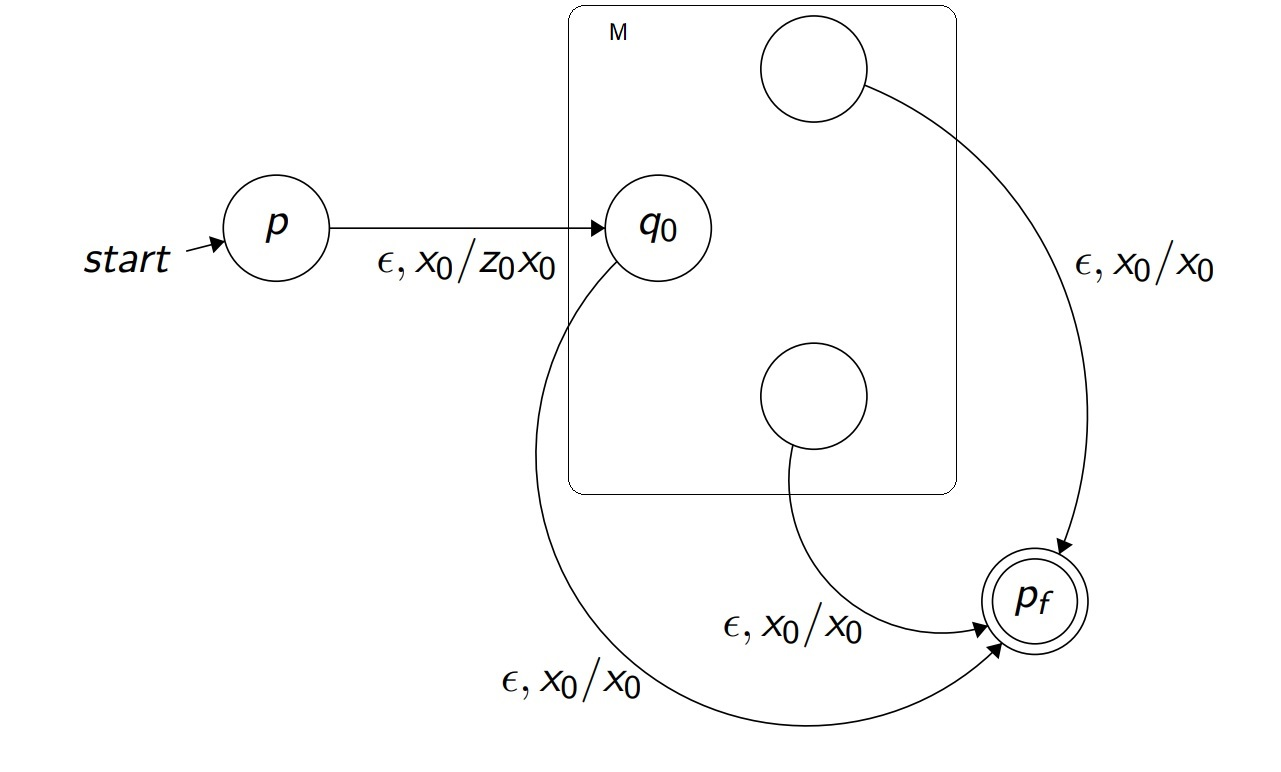
\includegraphics[scale=.3]{img4/m3}
			\caption{Transition diagram of M'}
		\end{figure}
	\end{center}
\end{frame}
\begin{frame}{ Equivalence of Acceptance by Final State and Empty Stack}
	\textbf{CASE 2:} PDA $M$ accepts by final state  (acceptance by  final state ($M$)  to acceptance by empty stack. ($M_1$
	))
	\begin{block}{Theorem}
		If $L = L(M)$ for some PDA $M = (Q, \Sigma, \Gamma, \delta_N, q_0, Z_0,f)$ then there is a PDA $M_1$ such that $L = N(M_1)$
	\end{block}
\textbf{Proof:}
\begin{itemize}
	\item Assume that PDA M accepts a language L by reaching a final state after processing an input string. 
	\item To show equivalence, we will construct another PDA, $M_1$, that accepts the same language L using an empty stack.
	\item To do this, we introduce two new states,$p_0$ and $p$ and a new stack symbol $x_0$ not in the original stack alphabet of M.
\end{itemize}
\end{frame}
\begin{frame}{ Equivalence of Acceptance by Final State and Empty Stack}
	\textbf{Proof cont..}
	\begin{itemize}
		\item The new PDA $M_1$ contains all the transitions of $M$, and in addition, it includes some more transitions:
		\begin{itemize}
			\item $\delta_1(p_0,\epsilon,x_0)=(q_0,z_0x_0)$ This transition allows $M_1$ to enter the initial
			configuration of $M$ with the bottom-of-stack marker $x_0$ below the
			symbols of $M’s$ stack.
			\item For every accepting state $q\in F$ in PDA M, add an $\epsilon$-transition from $q$ to p in PDA $M_1$.
			$$\delta_1(q,\epsilon,\gamma) \ contain\   (p,\epsilon)$$ where $\gamma$ any stack symbol
			\item For all stack symbol $\gamma \in \Gamma \cup \{x_0\}$
				$$\delta_1(p,\epsilon,\gamma) \ contain\   (p,\epsilon)$$
		\end{itemize}
	\end{itemize}
\end{frame}
\begin{frame}{ Equivalence of Acceptance by Final State and Empty Stack}
	\textbf{Proof cont..}
	\begin{itemize}
		\item Pushing $z_0$ onto the stack, $p_0$ enters the state $q_0$, which is the initial state of PDA M. Then, after consuming its input $w$, PDA $M$ enters one of its final states. \item To construct PDA $M1$, for each accepting state $q$ in PDA $M$, we add a transition to the new state $p$ on epsilon ($\epsilon$) with any stack symbol and delete that stack symbol. This process allows PDA $M_1$ to simulate the behavior of PDA $M$ and recognize when $M$ empties its stack.
		
		\item As a result, whenever PDA M enters a final state after consuming the input $w$, PDA $M_1$ will empty its stack after processing the same input $w$.
		\item  Hence, PDA $M_1$ accepts the same language L as PDA $M$, proving the equivalence of acceptance by final state and empty stack.
		
		
	\end{itemize}
\end{frame}
\begin{frame}{ Equivalence of Acceptance by Final State and Empty Stack}
		\textbf{Proof cont..}
\begin{center}
	\begin{figure}
		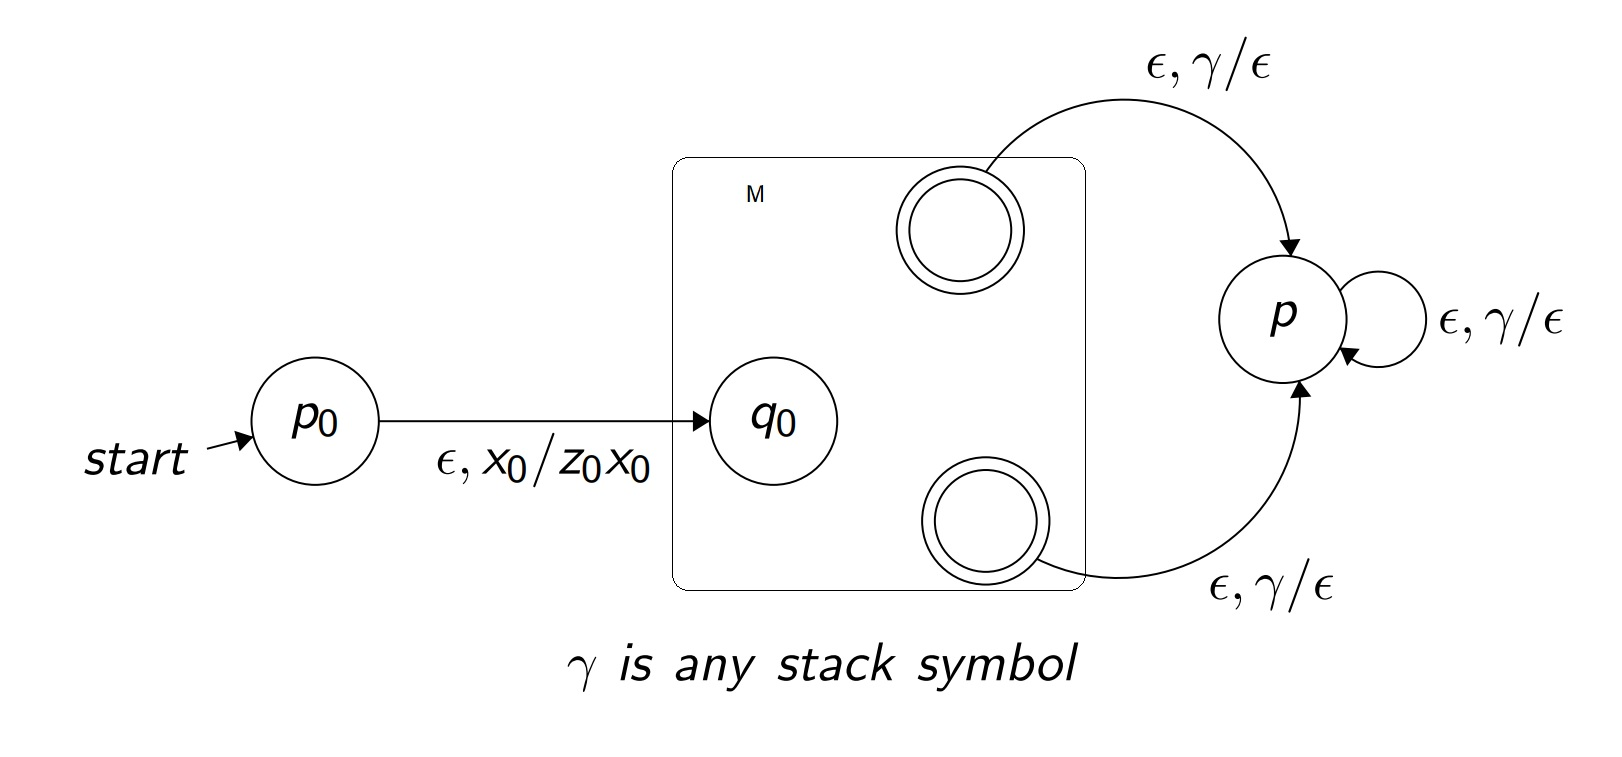
\includegraphics[scale=.3]{img4/m4}
		\caption{Transition diagram of M'}
	\end{figure}
\end{center}
\end{frame}
\section{Deterministic PDA (DPDA)}
\begin{frame}{Deterministic PDA (DPDA)}
	\textbf{Deterministic PDA (DPDA)}
	\begin{itemize}
		\item A PDA is said to be deterministic if all derivation(ID) in the design has to give only single move.
		\begin{itemize}
		\item That is the PDA is deterministic in the sense that at most one move is possible the given state, input symbol and stack symbol
		\end{itemize}
	\end{itemize}
	\textbf{Formally we say a PDA $M=(Q,\Sigma,\delta,\Gamma,q_0,z_0,F)$ is deterministic if}
	\begin{enumerate}
		\item $\delta (q,a,X)$ has at most one member for any $q \in Q, a \in \Sigma \cup \epsilon $ and $X \in \Gamma$
		\item If $\delta (q,a,X)$ is nonempty, for some $a \in \Sigma$ then $\delta (q,\epsilon,X)$ must be empty
 		\end{enumerate}
 	$^*$The DPDA’s accept a class of languages that is between the regular languages and the CFL’s.
\end{frame}
\begin{frame}{Deterministic PDA (DPDA)}

	\textbf{Example:}
	\begin{itemize}
		\item Consider the language $L = \{0^n1^n|n \geq 1\}$. It turns out that this language can be recognized by a deterministic PDA.
		 \begin{enumerate}
		 	\item The PDA starts in the initial state and begins to read the input string.
			
			\item While reading consecutive 0's, it pushes them onto the stack, effectively storing the count of 0's encountered.
			
			\item Upon encountering a 1, the PDA transitions to another state, where it starts popping the 0's from the stack each time it reads a 1.
			
			\item If the PDA tries to pop more 0's than the number of 0's it has encountered while reading the input, it reaches a state where the stack is empty before consuming all the input. In this case, the PDA halts and rejects the input since it cannot be in the form $0^m 1^m$, where m is the number of 0's encountered.
			
			\item If the PDA successfully pops all the 0's from the stack, and the entire input has been read, it reaches the initial symbol at the bottom of the stack.
			
			\item When the PDA reaches the initial symbol at the bottom of the stack after reading the entire input, it accepts the input since the number of 0's and 1's is equal and in the correct order.
		\end{enumerate}
	\end{itemize}
\end{frame}
\begin{frame}{Deterministic PDA (DPDA)}
	\textbf{Example:}
		\begin{figure}
		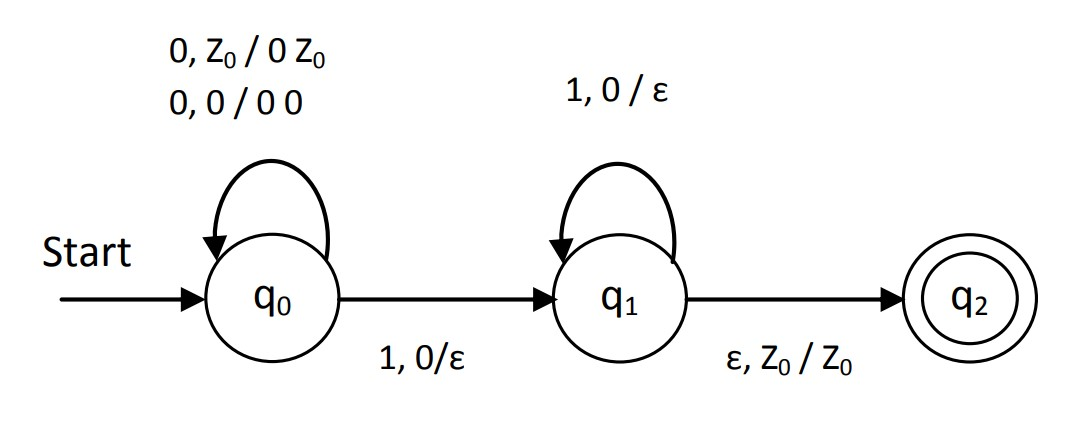
\includegraphics[scale=.3]{img4/m5}
		\caption{	Deterministic PDA accepting $\{0^n1^n| n > 1\}$}
	\end{figure}
\end{frame}
\begin{frame}{Deterministic PDA (DPDA)}
	\begin{figure}
		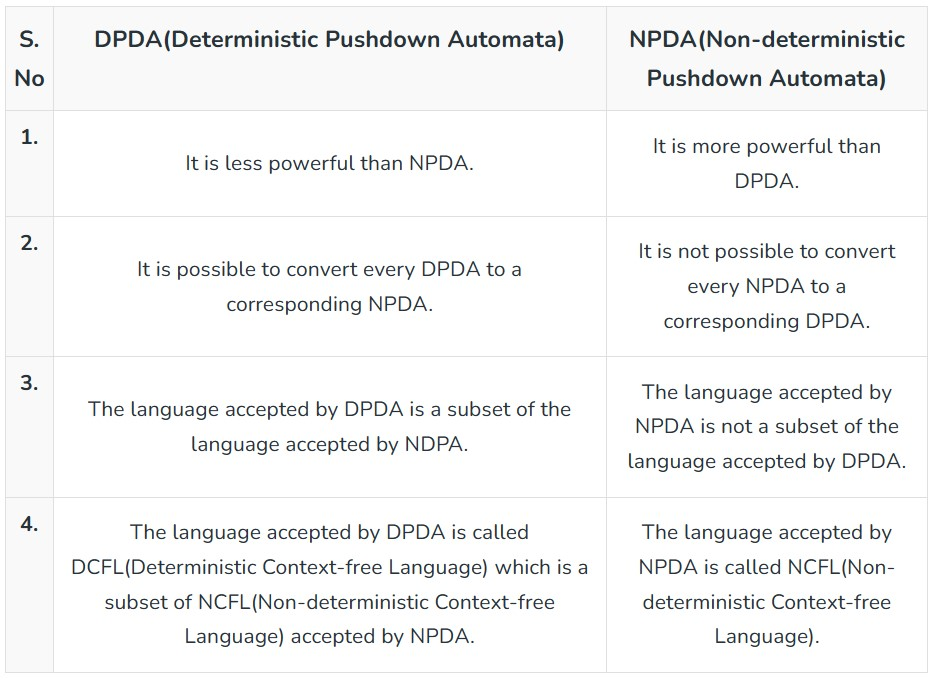
\includegraphics[scale=.5]{img4/m9}
		\caption{Difference Between NPDA and DPDA}
	\end{figure}
\end{frame}
\section{Equivalence of PDA's and CFL's }
\begin{frame}{Equivalence of PDA's and CFL's }
	The goal is to prove that the following three classes of the languages are all the same
	class.
	\begin{enumerate}
		\item The context-free languages (The language defined by CFG’s).
		\item The languages that are accepted by empty stack by some PDA.
	\item The languages that are accepted by final state by some PDA.

	\end{enumerate}
		\begin{figure}
		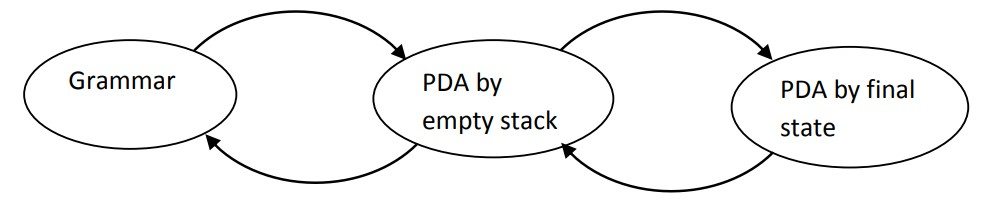
\includegraphics[scale=.5]{img4/m6}
		\caption{Organization of constructions showing equivalence of three ways of defining the CFL’s}
	\end{figure}
We have already shown that (2) and (3) are the same. Now, we prove that (1) and
(2) are same.

\end{frame}
\subsection{Conversion of CFG to PDA}
\begin{frame}{Conversion of CFG to PDA}
	\textbf{Conversion of CFG to PDA}
	\begin{itemize}
		\item If $L$ is a context-free language, then there exists a PDA M such that $L = N(M)$.
	\end{itemize}
\textbf{Procedure}
\begin{itemize}
	\item Let $L=L(G)$, where $G=(V, T,P,S)$ is a context free grammar. 
	\item We construct a PDA $M=M= (Q,\Sigma,\Gamma,\delta,q_0,z_0,F)$ such that $L(M)=L(M)$ by empty stack
	\item The machine constructed has only one state q
	\item All terminals are the input Symbol
	\item The set of nonterminals and the set of terminals as its stack symbol

\end{itemize}
\end{frame}
\begin{frame}{Conversion of CFG to PDA}
	\textbf{Procedure cont..}
	\small
	\begin{itemize}
		\item  $M=M= (Q,\Sigma,\Gamma,\delta,q_0,z_0,F)$ 
		\item where 
		\begin{eqnarray*}
			Q&=&\{q\}\\
			\Sigma&=&T\\
			\Gamma &=& V \cup T\\
			q_0&=&q\\
			z_0&=&S\\
			F&=&\phi\\
		\end{eqnarray*}
	Where $\delta$ is defined by the following rules	
	\begin{enumerate}
		\item If $A\rightarrow \beta$ is in P $\beta \in (V \cup T)^*$ Then 
		\begin{itemize}
			\item $\delta(q,\epsilon,A)$ contain $(q,\beta)$
		\end{itemize}
	\item For each $a\in T$
	\begin{itemize}
		\item $\delta(q,a,a)$ contains $(q,\epsilon)$
	\end{itemize}
	\end{enumerate}
	\end{itemize}
\end{frame}
\begin{frame}{Conversion of CFG to PDA}
	\textbf{Example:}Construct a pda M equivalent to the following context free grammar:
	\begin{eqnarray*}
		S&\rightarrow&0BB\\
		B&\rightarrow&0S|1S|0.
\\
	\end{eqnarray*}
Test whether $010^4$ is in $N(M)$.\\
\textbf{Solution:}
Define pda A as follows:
$$A=(\{q\},\{0,1\}, \delta,\{S,B,0,1\},q, S, \phi)$$
$\delta$ is defined by the following rules:
\begin{eqnarray*}
	&R1:& \delta(q, \epsilon, S)=\{(q,0BB)\}\\
	&R2:& \delta(q, \epsilon, B)=\{(q,0S),(q,1S),(q,0)\}\\
	&R3:& \delta(q, 0,0)=\{( q, \epsilon)\}\\
	&R4:& \delta(q, 1,1)=\{( q, \epsilon)\}\\
\end{eqnarray*}
\end{frame}
\begin{frame}{Conversion of CFG to PDA}
	\textbf{String Checking }
	\begin{eqnarray*}
		(q,010^4,S) 
		&\vdash& (q, 010^4, 0BB) \ \ \ by Rule R1 \\
		&\vdash& (q, 10^4, BB) \ \ \ by Rule R3 \\
		&\vdash& (q, 10^4,1SB) \ \ \ by Rule R2 \\
		&\vdash& (q, 0^4, SB) \ \ \ by Rule R4 \\ 
		&\vdash& (q, 0^4, 0BBB) \ \ \ by Rule R1 \\
		&\vdash& (q, 0^3,BBB) \ \ \ by Rule R3 \\
		&\vdash^*&(q, 0^3,000) \ \ \ by Rule R2 \\ 
		&\vdash^*&(q, \epsilon , \epsilon)  \ \ \ by Rule R3 \\ 
	\end{eqnarray*}
\end{frame}
\subsection{Conversion of PDA to CGF}
\begin{frame}{Conversion of PDA to CGF}
\textbf{Conversion of PDA to CGF}
\begin{itemize}
	\item Will do this in two steps 
	\begin{enumerate}
		\item Every NPDA can be simulated by an NPDA with one state
		\item Every NPDA with one state has an equivalent CFG.
	\end{enumerate}
\end{itemize}
\end{frame}
\begin{frame}{Conversion of PDA to CGF}
	\textbf{Converting many-state PDA to one-state PDA}
	\begin{itemize}
		\item Let’s say $P$ is a many state PDA with transition relation $\delta$.
		\item We’ll create a single	state PDA P1 with transition relation $\delta_1$.
		\item  The stack symbols of P1 look like
		$[pXq]$ where p and q are states of P and X is a stack symbol from P 
		\item P1 has only one state which we’ll call 1 for
		distinction. 
		\item For each transition in $\delta$, create one or more transitions in $\delta_1$.
	\end{itemize}
\end{frame}
\begin{frame}{Conversion of PDA to CGF}
	\begin{itemize}
		\item[1]  $\delta$ pops a symbol (and moves from p to q)
		\begin{eqnarray*}
			\delta(p, a, X) = \{(q,\epsilon)\}
			&\implies&
			\delta_1(1, a, [pXq]) = \{(1,\epsilon)\}
\\
		\end{eqnarray*}
	\item[2] $\delta$ replaces a symbol
\begin{eqnarray*}
	\delta(p, a, X) = \{(q, Y )\}
	&\implies&
	\forall_b \delta_1(1, a, [pXb]) = \{(1, [qY b])\} \\
\end{eqnarray*}
\item[3] $\delta$ pushes 2 or more symbols
\begin{eqnarray*}
	\delta(p, a, X) = \{(q, Y Z)\}
	\implies
	\forall_g, b \delta_1(1, a, [pXb]) = \{(1, [qY g][gZb])\}
\\
\end{eqnarray*}
	\end{itemize}
\small
$^*$If $\delta$ pushes more symbols, e.g. $WXYZ$, then we must make a guess
for each symbol, and the RHS will look like: $[qW g_1][g_1Xg_2][g_2Y g_3][g_3Zb]$
\end{frame}
\begin{frame}{Conversion of PDA to CGF}
	\textbf{Example}
	\begin{itemize}
		\item Let P be a PDA that accepts $\{0^n10^n|n \geq 1\}$ and has three states:
		\begin{itemize}
			\item State p reads 0’s from the input and pushes them onto the stack. It may
			stay in state p or move to state q.
				\item State q reads a single 1 from the input and moves to state r.
			\item State r reads 0’s from the input and pops 0’s from the stack.
		\end{itemize}
	\item $\delta$ looks like:
	\end{itemize}
\begin{eqnarray*}
	\delta(p, 0, Z0) & = & \{(p, 0Z0),(q, 0Z0)\} \\
	\delta(p, 0, 0) & = & \{(p, 00),(q, 00)\} \\
	\delta(q, 1, 0)  &= & \{(r, 0)\} \\
	\delta(r, 0, 0) & = & \{(r, \epsilon)\} \\
	\delta(r, 0, Z0) & = & \{(r, \epsilon)\} \\
\end{eqnarray*}
\end{frame}
\begin{frame}{Conversion of PDA to CGF}
	\textbf{Example cont..}\\
	Here are the stack symbols of P1:
\begin{itemize}
	\item[*] [p0p], [p0q], [p0r] \item[*] [p1p], [p1q], [p1r] \item[*] [p$Z_0$p], [p$Z_0$q], [p$Z_0$r] 
	\item[*] [q0p], [q0q], [q0r] \item[*] [q1p], [q1q], [q1r] \item[*] [q$Z_0$p], [q$Z_0$q], [q$Z_0$r] \item[*]
	[r0p], [r0q], [r0r] \item[*] [r1p], [r1q], [r1r] \item[*] [r$Z_0$p], [r$Z_0$q], [r$Z_0$r] 
\end{itemize}
\end{frame}
\begin{frame}{Conversion of PDA to CGF}
	\small
Here are three examples of transitions in $\delta$ and the transitions in $\delta_1$ that they generate.
\begin{itemize}
	\item[1]  $\delta(p, 0, 0) \rightarrow (q, 00)$
\begin{eqnarray*}
\delta_1(1, 0, [p0p]) &=& \{(1, [q0p][p0p]),(1, [q0q][q0p]),(1, [q0r][r0p])\} \\
\delta_1(1, 0, [p0q]) &=& \{(1, [q0p][p0q]),(1, [q0q][q0q]),(1, [q0r][r0q])\} \\
\delta_1(1, 0, [p0r]) &=& \{(1, [q0p][p0r]),(1, [q0q][q0r]),(1, [q0r][r0r])\} \\
\end{eqnarray*}
\item[2] $\delta(q, 1, 0) \rightarrow (r, 0)$
\begin{eqnarray*}
	\delta_1(1, 1, [q0p]) &=& \{(1, [r0p])\} \\
	\delta_1(1, 1, [q0q]) &=& \{(1, [r0q])\} \\
	\delta_1(1, 1, [q0r]) &=& \{(1, [r0r])\} \\
\end{eqnarray*}
\item $\delta(r, 0, 0) \rightarrow (r, \epsilon)$
\begin{eqnarray*}
\delta_1(1, 0, [r0r]) &=& {(1, \epsilon)} \\
\end{eqnarray*}
\end{itemize}
\end{frame}
\begin{frame}{Conversion of PDA to CGF}
	\textbf{Single state PDA to grammar G}
	\begin{itemize}
		\item For a single State PDA $N = (Q, \Sigma, \Gamma, \delta, q, Z_0),$ we construct a grammar	$G = (V,T,P,S)$, such that
		\begin{itemize}
			\item $L(G) = L(N)$, where $V = \Gamma, T = \Sigma \ and\  S = Z_0$. the following rules outline the set of productions, P :
			\begin{eqnarray*}
				For\  every\  (q, a, Z)\  &=&\  (q, \gamma),\  we\  add\  Z \rightarrow a\gamma, \ where\ \\
				&\  & a \in \Sigma \cup \{\epsilon\},	Z \in \Gamma, \gamma \in \Gamma^* \\
			\end{eqnarray*}
		\end{itemize} 
	\end{itemize}
\end{frame}
\begin{frame}{Conversion of PDA to CGF}
	\textbf{Example:}Consider the PDA $P_N = (\{q\}, \{0, 1\}, \{Z, A, B\}, \delta_N, q, Z)$ in Figure The corresponding context-free grammar $G = (V, \{0, 1\}, P, S)$ is given by:
	\begin{figure}
		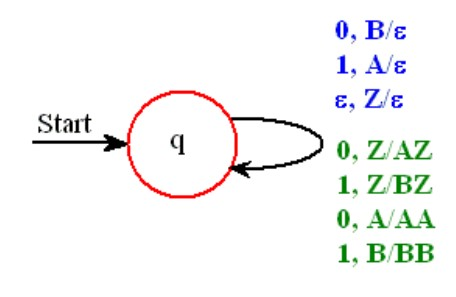
\includegraphics[scale=.5]{img4/m7}
	%	\caption{Block diagram of a Pushdown Automata}
	\end{figure}
\textbf{Solution:}
\begin{itemize}
	\item $V = \{S, Z, A, B\}$.
\end{itemize}
\end{frame}
\begin{frame}{Conversion of PDA to CGF}
	\textbf{Example cont..}\\
	P:
\begin{eqnarray*}
S &\rightarrow& Z \\
\end{eqnarray*}
\begin{eqnarray*}
Z &\rightarrow& 0AZ\  (\ since\  \delta_N (q, 0, Z) \ contains\  (q, AZ)) \\
\end{eqnarray*}
\begin{eqnarray*}
	Z &\rightarrow& 1BZ \ (\ since\  \delta_N (q, 1, Z) \ contains\  (q, BZ)) \\
\end{eqnarray*}
\begin{eqnarray*}
	A &\rightarrow& 0AA \ (\ since\  \delta_N (q, 0, A) \ contains\  (q, AA)) \\
\end{eqnarray*}
\begin{eqnarray*}
	B &\rightarrow& 1BB\  (\ since\  \delta_N (q, 1, B) \ contains\  (q, BB)) \\
\end{eqnarray*}

\end{frame}
\begin{frame}{Conversion of PDA to CGF}
	\textbf{Example cont..}\\
\begin{eqnarray*}
	A &\rightarrow& 1\  (\ since\  \delta_N (q, 1, A) \ contains\  (q, \epsilon))\\
\end{eqnarray*}
\begin{eqnarray*}
	B &\rightarrow& 0\  (\ since\  \delta_N (q, 0, B) \ contains\  (q, \epsilon)) \\
\end{eqnarray*}
\begin{eqnarray*}
	Z &\rightarrow& \epsilon\  (\ since\  \delta_N (q, \epsilon, Z) \ contains\  (q, \epsilon))\\
\end{eqnarray*}
\end{frame}
\section{Pumping Lemma for context-free languages}
\begin{frame}{Pumping Lemma for context-free languages}
	There is a pumping lemma for CFLs similar to the one for regular sets. It 
	can be used in the same way to show that certain sets are not context-free. \\
	\textbf{Pumping Lemma for context-free languages}
	\begin{itemize}
		\item Let L be any CFL. Then there is a constant n, depending only on $L,$ such 
		that if $z$ is in L and $| z | \geq n,$ then we may write $z = uvwxy$ such that
		\begin{enumerate}
			\item $|vx| \geq 1,i.e\ vx \neq \epsilon$
			\item $|vwx|\leq n, \ and$
			\item for all $i\geq 0, uv^iwx^iy$ is in $L$.
		\end{enumerate}
	\end{itemize}
\begin{figure}
	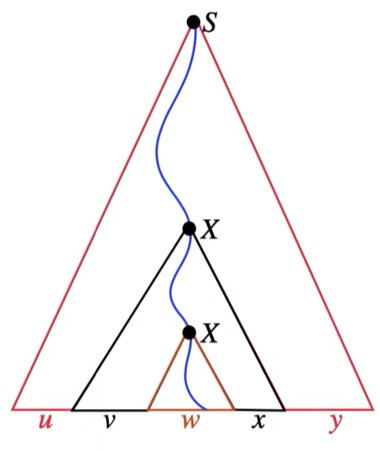
\includegraphics[scale=.4]{img4/m8}
	%\caption{Block diagram of a Pushdown Automata}
\end{figure}
\end{frame}
\begin{frame}{Pumping Lemma for context-free languages}
	\textbf{Example:}
	Consider the language $L = \{a^p | p\ is\ prime\}$. Suppose $L$ were context free and let 
	$n$ be the constant. $n \in N$
	\begin{itemize}
	%	\item Assume that the language L is context free language
		\item $L=\{a,a^3,a^5,a^7,......\}$
		\begin{itemize}
			\item Consider $z = a^5.$ 
			\begin{itemize}
				\item $\big |z \big | =5\ \ 5\geq n$
			\end{itemize}
			\item Write $z = uvwxy$ so as to satisfy the conditions of the pumping lemma.
			\begin{enumerate}
				\item $|vx| \geq 1,i.e\ vx \neq \epsilon$
				\item $|vwx|\leq n, \ and$
				\item for all $i\geq 0, uv^iwx^iy$ is in $L$.
			\end{enumerate}
		\end{itemize}
		Assume $u=a,v=a,w=a,x=a,y=a$ 
	\item	put i=3: then $uv^iwx^iy$ become
	\begin{itemize}
		\item $a(a)^3a(a)^3a$ = $aaaaaaaaa$
		\item   $ \big | aaaaaaaaa \big | =9$, 9 is not a prime number, which is not belong to L, so this contradicts our assumption
		\item So L is not context free.
	\end{itemize}
	\end{itemize}
\end{frame}

%\begin{frame}{Pumping Lemma for context-free languages}
%	\textbf{Example:}
%	Consider the language $L = \{a^ib^ic^i | \geq 1\}$. Suppose $L$ were context free and let 
%	$n$ be the constant.
%	\begin{itemize}
%		\item Consider $z = a^nb^nc^n.$ Write $z = uvwxy$ so as to satisfy the conditions of the pumping lemma.
%		\item Since $|vwx| \leq n,$ it is not possible for $vx$ to contain instances of $a’s$ and $c’s$, 
%		because the rightmost $a$ is $n + 1$ positions away from the leftmost $c.$ 
%		\item If $v$ and $x$ consist of $a’s$ only, then $uwy$ (the string $uv^iwx^iy$ with $i = 0$) has n 
%		$b’s$ and n $c’s$ but fewer than n $a’s$ since $|vx|\geq 1.$
		
%		\item Thus, $uwy$ is not of the form $a^ib^ic^i$
%		. But by the pumping lemma $vwy$ is in $L,$ a
%		contradiction.
		
%		\item The cases where $v$ and $x$ consist only of $b’s$ or only of $c’s$ are disposed of
%		similarly.
%		\item If $vx$ has $a’s$ and $b’s$, then $uwy$ has more $c’s$ than $a’s$ or $b’s,$ and again it is
	%	not in L.
%		\item If $vx$ contains $b’s$ and $c’s$, a similar contradiction results.
%		\item We conclude that L is not a context-free language.
%	\end{itemize}
%\end{frame}
\section{Closure Properties of Context Free Languages}
\begin{frame}{Closure Properties of Context Free Languages}
\textbf{Closure Properties of Context Free Languages}
\begin{itemize}
	\item A CFL is basically a set of strings
	\item \textbf{Closure properties} of any set $S$ is the operations which take element/elements of $S$ as input and produce an element of $S$ as output
	\item Thus, closure properties of CFLs are those set operations which take CFLs/CFL as input and produces a CFL as output
\end{itemize}
\textbf{Closure Properties}
\begin{enumerate}
	\item Context-free languages are closed under union, concatenation and 
	Kleene closure.
	\item The context-free languages are closed under substitution.
	\item The CFL’s are closed under homomorphism.
	\item The CFL’s are closed under inverse homomorphism.
	\item The CFL’s are not closed under intersection.
	\item The CFL’s are not closed under complementation.
	\item If L is a CFL and R is a regular set, then $L\cap R$ is a CFL
\end{enumerate}
\end{frame}
\begin{frame}{Closure Properties of Context Free Languages}
	\textbf{Theorem:} CFLs are closed under union
	\begin{itemize}
		\item If $L_1$ and $L_2$ are CFLs, then $L_1 \cup L_2$ is a CFL.
	\end{itemize}
\proofname 
\begin{itemize}
	\item Let L1 and L2 be generated by the CFG, $G_1 = (V_1, T_1, P_1, S_1)$ and
	$G_2 = (V_2, T_2, P_2, S_2)$, respectively.
	\item Without loss of generality, subscript each nonterminal of $G_1$ with a 1,
	and each nonterminal of $G_2$ with a 2 (so that $V_1 \cap V_2 = \phi)$.
	\item Define the CFG, $G,$ that generates $L_1 \cup L_2$ as follows:
	$G = (V_1 \cup V_2 \cup \{S\}, T_1 \cup T_2, P_1 \cup P_2 \cup \{S \rightarrow S_1 | S_2\}, S).$
	\item A derivation starts with either $S \implies S_1\  or\  S \implies S_2.$
	\item Subsequent steps use productions entirely from $G_1$ or entirely from
	$G_2$.
	\item Each word generated thus is either a word in $L_1$ or a word in $L_2$.

\end{itemize}
\end{frame}
\begin{frame}{Closure Properties of Context Free Languages}
	\textbf{Example:}
	\begin{itemize}
		\item Let $L1$ be Palindrome, defined by
		\begin{itemize}
			\item $S_1\rightarrow aS_1a | bS_1b | a | b | \epsilon$
		\end{itemize}
	\item Let L2 be $\{a^nb^n	|n \geq 0\}$ defined by:
	\begin{itemize}
		\item $S_2\rightarrow aS_2b | \epsilon$
	\end{itemize}
\item Then the union language is defined by:
\begin{eqnarray*}
	S &\rightarrow& S_1 | S_2 \\
	S_1 &\rightarrow& aS_1a | bS_1b | a | b | \epsilon \\
	S_2 &\rightarrow& aS_2b | \epsilon \\
\end{eqnarray*}
	\end{itemize}
\end{frame}
\begin{frame}{Closure Properties of Context Free Languages}
	\textbf{Theorem:} CFLs are closed under concatenation
	\begin{itemize}
		\item If $L_1 \ and \ L_2$ are CFLs, then $L_1L_2$ is a CFL.
	\end{itemize}
\proofname
\begin{itemize}
	\item Let $L_1$ and $L_2$ be generated by the CFG, $G_1 = (V_1, T_1, P_1, S_1)$ and
	$G_2 = (V_2, T_2, P_2, S_2),$ respectively.
	\item Without loss of generality, subscript each nonterminal of $G_1$ with a 1,
	and each nonterminal of $G_2$ with a 2 (so that $V_1 \cap V_2 = \phi).$
	\item Define the CFG, $G,$ that generates $L_1L_2$ as follows:
	$G = (V_1 \cup V_2 \cup \{S\}, T_1 \cup T_2, P_1 \cup P_2 \cup \{S \rightarrow S_1S_2\}, S).$
	\item Each word generated thus is a word in $L_1$ followed by a word in $L_2$.

\end{itemize}
\end{frame}
\begin{frame}{Closure Properties of Context Free Languages}
	\textbf{Example} 
	\begin{itemize}
		\item Let L1 be Palindrome, defined by:
		\begin{itemize}
			\item 	$S_1 \rightarrow aS_1a | bS_1b | a | b | \epsilon$
		\end{itemize}
		\item Let L2 be $\{a^nb^n	|n \geq 0\}$ defined by:
		\begin{itemize}
			\item $S_2 \rightarrow aS_2b | \epsilon$
		\end{itemize}
		\item Then the concatenation language is defined by:
	\begin{eqnarray*}
			S &\rightarrow& S_1S_2 \\
		S_1 &\rightarrow& aS_1a | bS_1b | a | b | \epsilon \\
		S_2 &\rightarrow& aS_2b | \epsilon \\
	\end{eqnarray*}
	\end{itemize}
\end{frame}
\begin{frame}{Closure Properties of Context Free Languages}
	\textbf{Theorem:} CFLs are closed under Kleene star
	\begin{itemize}
		\item If $L_1$ is a CFL, then $L_1^* $is a CFL.
	\end{itemize}
\proofname 
\begin{itemize}
	\item Let $L_1$ be generated by the CFG, $G_1 = (V_1, T_1, P_1, S_1)$.
		\item Without loss of generality, subscript each nonterminal of $G_1$ with a 1.
		\item Define the CFG, G, that generates $L_1^*$	as follows:
		\begin{itemize}
			\item 	$G = (V_1 \cup \{S\}, T_1, P_1 \cup \{S \rightarrow S_1S | \epsilon \}, S).$
		\end{itemize}
		\item Each word generated is either $\epsilon$  or some sequence of words in $L_1$.
		\item Every word in $L_1^*$
	(i.e., some sequence of 0 or more words in $L_1$) can be generated by G.
\end{itemize}
\end{frame}
\begin{frame}{Closure Properties of Context Free Languages}
	\textbf{Example}
	\begin{itemize}
		 \item Let $L_1$ be $\{a^nb^n|n \geq 0\}$ defined by:
		\item $S \rightarrow aSb | \epsilon$
		\item Then $L_1^*$	is generated by:
	\begin{eqnarray*}
		S&\rightarrow& S_1S | \epsilon\\
		S_1&\rightarrow& aS_1b | \epsilon\\
	\end{eqnarray*}
		None of these example grammars is necessarily the most compact CFG
		for the language it generates.
	\end{itemize}
\end{frame}
\begin{frame}{Closure Properties of Context Free Languages}
	\textbf{Theorem:} CFLs are not closed under intersection
	\begin{itemize}
		\item If $L_1$ and $L_2$ are CFLs, then $L_1 \cap L_2$ may not be a CFL
	\end{itemize}
\proofname
\begin{itemize}
	\item $L_1 = \{a^nb^na^m | n, m \geq 0\}$ is generated by the following CFG:
	\begin{eqnarray*}
		S &\rightarrow& XA \\
		X &\rightarrow& aXb|\epsilon \\
		A &\rightarrow& Aa|\epsilon 
	\end{eqnarray*}
\item $L_2 = \{a^nb^ma^m | n, m \geq 0\}$ is generated by the following CFG:
\begin{eqnarray*}
S & \rightarrow & AX \\
X & \rightarrow & aXb | \epsilon \\
A & \rightarrow & Aa | \epsilon \\
\end{eqnarray*}
\item $L_1 \cap L_2 = \{a^nb^na^n| n \geq 0\}$, which is known not to be a CFL
(pumping lemma).

\end{itemize}
\end{frame}
\begin{frame}{Closure Properties of Context Free Languages}
	\textbf{Theorem:} CFLs are not closed under complement
	\begin{itemize}
		\item If $L_1$ is a CFL, then $\bar{L_1}$ may not be a CFL.
	\end{itemize}
	\proofname
	\begin{itemize}
		\item Assume the complement of every CFL is a CFL
		\item Let $L_1$ and $L_2$ be 2 CFLs.
		\item Since CFLs are close under union, and we are assuming they are closed
		under complement, $\overline{\bar{L_1} \cup \bar{L_2}} = L1 \cap L2$
		is a CFL.
	\item However, we know there are CFLs whose intersection is not a CFL.
	\item Therefore, our assumption that CFLs are closed under complement is
	false.
	\end{itemize}
\end{frame}
\begin{frame}{Closure Properties of Context Free Languages}
	\textbf{Example}
		This does not mean that the complement of a CFL is never a CFL
		\begin{itemize}
			\item Let $L_1 = \{a^nb^na^n|n \geq 0\}$, which is not a CFL.
			\item $\bar{L_1}$ is a CFL.
			\item We show this by constructing it as the union of 5 CFLs.
			\begin{itemize}
				\item $M_{pq} = (a^+)(a^nb^n)(a^+) = \{a^pb^qa^r| p > q\}$
				\item $M_{qp} = (a^nb^n)(b^+)(a^+) = \{a^pb^qa^r| p < q\}$
				\item $M_{qr} = (a^+)(b^+)(b^na^n) = \{a^pb^qa^r| q > r\}$
				\item $M_{qr} = (a^+)(b^na^n)(a^+) = \{a^pb^qa^r| q < r\}$
				\item $M = a^+b^+a^+ =$ all words not of the form $a^pb^qa^r$
			\end{itemize}
		
			\item Let $L = M \cup M_{pq} \cup M_{qp} \cup M_{qr} \cup M_{qr}.$
			\item Since $M \subseteq L,\  L $contains only words of the form $a^pb^qa^r$
		\end{itemize}
\end{frame}
\begin{frame}{Closure Properties of Context Free Languages}
	\textbf{Example cont..}
\begin{itemize}
	\item $\bar{L}$ cannot contain words of the form $a^pb^qa^r$, where $p < q.$
	\item $\bar{L}$ cannot contain words of the form $a^pb^qa^r,$ where $p > q.$
	\item Therefore $\bar{L}$ only contains words of the form $a^pb^qa^r,$ where $p= q.$
	\item $\bar{L}$ cannot contain words of the form $a^pb^qa^r$, where $q < r.$
	\item $\bar{L}$ cannot contain words of the form $a^pb^qa^r$, where $q > r.$
	\item Therefore $\bar{L}$ only contains words of the form $a^pb^qa^r,$ where $q = r.$
	\item Since $p = q$ and $q = r, \ \bar{L}$ contains words of the form $a^nb^na^n,$ which	is not context-free.

\end{itemize}
\end{frame}
\begin{frame}{Closure Properties of Context Free Languages}
	\textbf{Theorem:} The intersection of a CFL and an RL is a CFL.
\begin{itemize}
	\item If$ L_1$ is a CFL and $L_2$ is regular, then $L_1 \cap L_2$ is a CFL
\end{itemize}
\proofname
\begin{itemize}
	\item We do this by constructing a PDA $I$ to accept the intersection that
	is based on a PDA A for $L_1$ and a FA $F$ for $L_2.$
	\item Convert A, if necessary, so that all input is read before accepting.
	\item Construct a set $Y$ of all $A’s$ states $y_1, y_2,...$, and a set $X$ of all $F’s$ states $x_1, x_2,....$
	\item Construct $\{(y, x) | \forall_y \in Y, \forall_x \in X\}$.
	\item The start state of $I$ is $(y_0, x_0),$ where $y_0$ is the label of $A’s$ start state,	and $x_0$ is $F’s$ initial state.
	\item Regarding the next state function, the $x$ component changes only
	when the PDA is in a READ state:
	\begin{itemize}
		\item If in $(y_i, x_j)$ and $y_i$	is not a READ state, its successor is $(y_k, x_j),$where $y_k$ is the appropriate successor of $y_i$		.
		\item If in $(y_i, x_j)$ and $y_i$is a READ state, reading a, its successor is$(y_k, x_l),$ where $y_k$ is the appropriate successor of $y_i$ on an a,
		$\delta(x_j	, a) = x_l$
	\end{itemize}
\end{itemize}
\end{frame}
\begin{frame}{Closure Properties of Context Free Languages}
		\begin{itemize}
		\item $I’s$ ACCEPT states are those where the $y$ component is ACCEPT
		and the $x$ component is final.
		\item If the $y$ component is ACCEPT and the $x$ component is not final, the
		state in $I$ is REJECT (or omitted, implying a crash).
	\end{itemize}

\end{frame}
\begin{frame}{Closure Properties of Context Free Languages}
		\textbf{Theorem:} Context free languages are closed under Homomorphism\\
		\textbf{Example:} 
	\begin{itemize}
		\item Suppose L is a CFL over alphabet $\Sigma$, and $h$ is a homomorphism on $\Sigma$.
		\item Let $s$ be the substitution that replaces each symbol a in $\Sigma$ by the language consisting of the one string that is $h(a)$
		\item i.e $ s(a)=\{h(a)\}$ for all a in $\Sigma$. then $h(L)=s(L)$
	\end{itemize}
	
\end{frame}
\end{document}